\documentclass[a4paper,fleqn,12pt]{article}
\usepackage{mathtools}
%\usepackage{amsthm}
\usepackage{amsmath}
%\usepackage{nccmath}
\usepackage{amssymb}
%\usepackage{amsfonts}
\usepackage{physics}
%\usepackage{dsfont}
%\usepackage{mathrsfs}
%\usepackage{slashed}    % Feynman slash notation, requires LuaLaTeX
%\usepackage[compat=1.1.0]{tikz-feynman}   % Feynman diagrams

%\usepackage{titling}
\usepackage{indentfirst}
%\usepackage[titletoc,title]{appendix}
%\renewcommand\appendixname{Apêndice}

\usepackage{bm}
%\usepackage{xcolor}
%\usepackage[dvipsnames]{xcolor}
\usepackage{cancel}

%\usepackage{xurl}
\usepackage{hyperref}
\usepackage{cite}

\usepackage{float}
\usepackage{graphicx}
\usepackage{tikz}
\usepackage{caption}
\usepackage{subcaption}

%%%%%%%%%%%%%%%%%%%%%%%%%%%%%%%%%%%%%%%%%%%%%%%%%%%

\newcommand{\eps}{\epsilon}
\newcommand{\vphi}{\varphi}
\newcommand{\cte}{\text{cte}}

\newcommand{\N}{\mathbb{N}}
\newcommand{\Z}{\mathbb{Z}}
\newcommand{\Q}{\mathbb{Q}}
\newcommand{\R}{\mathbb{R}}
\newcommand{\C}{\mathbb{C}}
\renewcommand{\P}{\mathbb{P}}
\renewcommand{\H}{\s{H}}

\newcommand{\0}{\vb{0}}
\newcommand{\1}{\mathds{1}}
\newcommand{\E}{\vb{E}}
\newcommand{\B}{\vb{B}}
\renewcommand{\v}{\vb{v}}
\renewcommand{\r}{\vb{r}}
\newcommand{\p}{\vb{p}}
\newcommand{\q}{\vb{q}}
\newcommand{\F}{\vb{F}}
\newcommand{\dtcp}{\delta_{\text{CP}}}

\newcommand{\s}[1]{\mathcal{#1}}
\renewcommand{\sl}[1]{\slashed{#1}}
\newcommand{\prodint}[2]{\left\langle #1 , #2 \right\rangle}
\newcommand{\cc}[1]{\overline{#1}}
\newcommand{\Eval}[3]{\eval{\left( #1 \right)}_{#2}^{#3}}

\newcommand{\unit}[1]{\; \mathrm{#1}}

\newcommand{\n}{\medskip}
\newcommand{\e}{\quad \mathrm{e} \quad}
\newcommand{\ou}{\quad \mathrm{ou} \quad}
\newcommand{\virg}{\, , \;}
\newcommand{\ptodo}{\forall \,}
\newcommand{\existe}{\exists \,}
\renewcommand{\implies}{\; \Rightarrow \;}
%\newcommand{\eqname}[1]{\tag*{#1}} % Tag equation with name

% MACROS
\newcommand{\dcp}{\delta_{\text{CP}}}


\title{\Huge{\textbf{Landau-Zener}}}
\author{Mateus Marques}

\begin{document}

\maketitle

\section{Filosofia}

\subsection{Caso \textit{muito fácil}}

Sempre escreveremos:
$$
\psi(t) = c_1(t) \ket{\uparrow} + c_2(t) \ket{\downarrow}.
$$

\n

Analisemos o caso muito fácil em que:
$$
\H =
\begin{bmatrix}
\alpha t/2 & 0 \\
0 & -\alpha t/2
\end{bmatrix}.
$$
As energias claramente são $E_{\pm} = \pm \frac{\alpha t}{2}$. Note que ao resolver a equação de Schrödinger:
$$
c_1(t) = c_1(0) \exp\qty(-\frac{i}{\hbar} \int_0^t E_+(u) \dd{u}),
$$
$$
c_2(t) = c_2(0) \exp\qty(-\frac{i}{\hbar} \int_0^t E_-(u) \dd{u}).
$$
De maneira que $\abs{c_1(t)}$ e $\abs{c_2(t)}$ são constantes (somente as fases deles ficam oscilando).

Em particular, se a condição inicial é tal que
$\psi_{\text{inicial}} = \begin{bmatrix} 1 \\ 0 \end{bmatrix}$, temos que a energia é \textit{definitivamente} $E_+$ para sempre.

\begin{figure}[H]
\centering
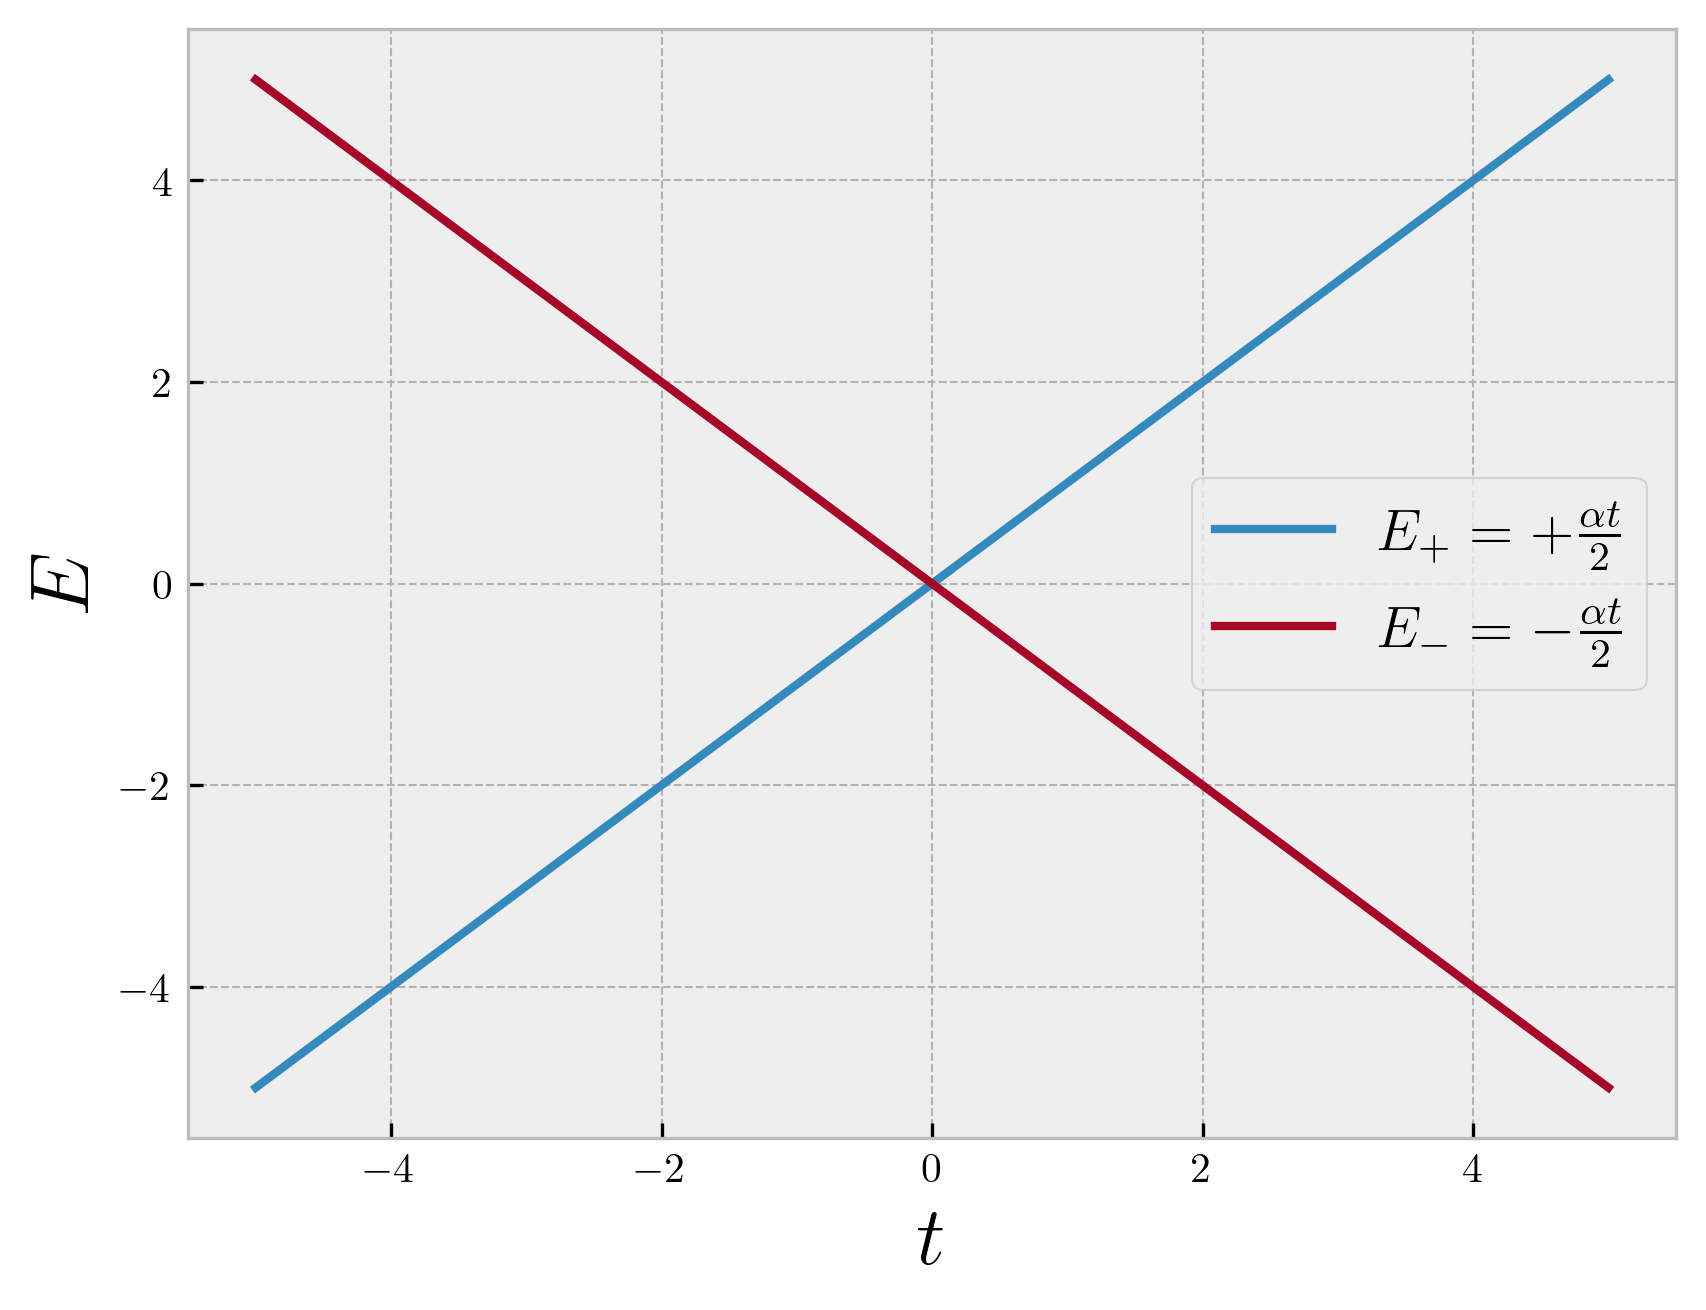
\includegraphics[scale=0.8]{figures/nogap.png}
\caption{Energias do problema muito fácil.}
\label{fig:nogap}
\end{figure}

\pagebreak

\subsection{Caso \textit{só fácil}}

Agora vamos supor a existência de um termo que não mais torna o $\H$ diagonal:
$$
\H =
\begin{bmatrix}
\alpha t/2 & \Delta/2 \\
\Delta^*/2 & -\alpha t/2
\end{bmatrix}.
$$
As energias agoram são $E_{\pm} = \pm \frac{1}{2} \sqrt{(\alpha t)^2 + \abs{\Delta}^2}$.
\begin{figure}[H]
\centering
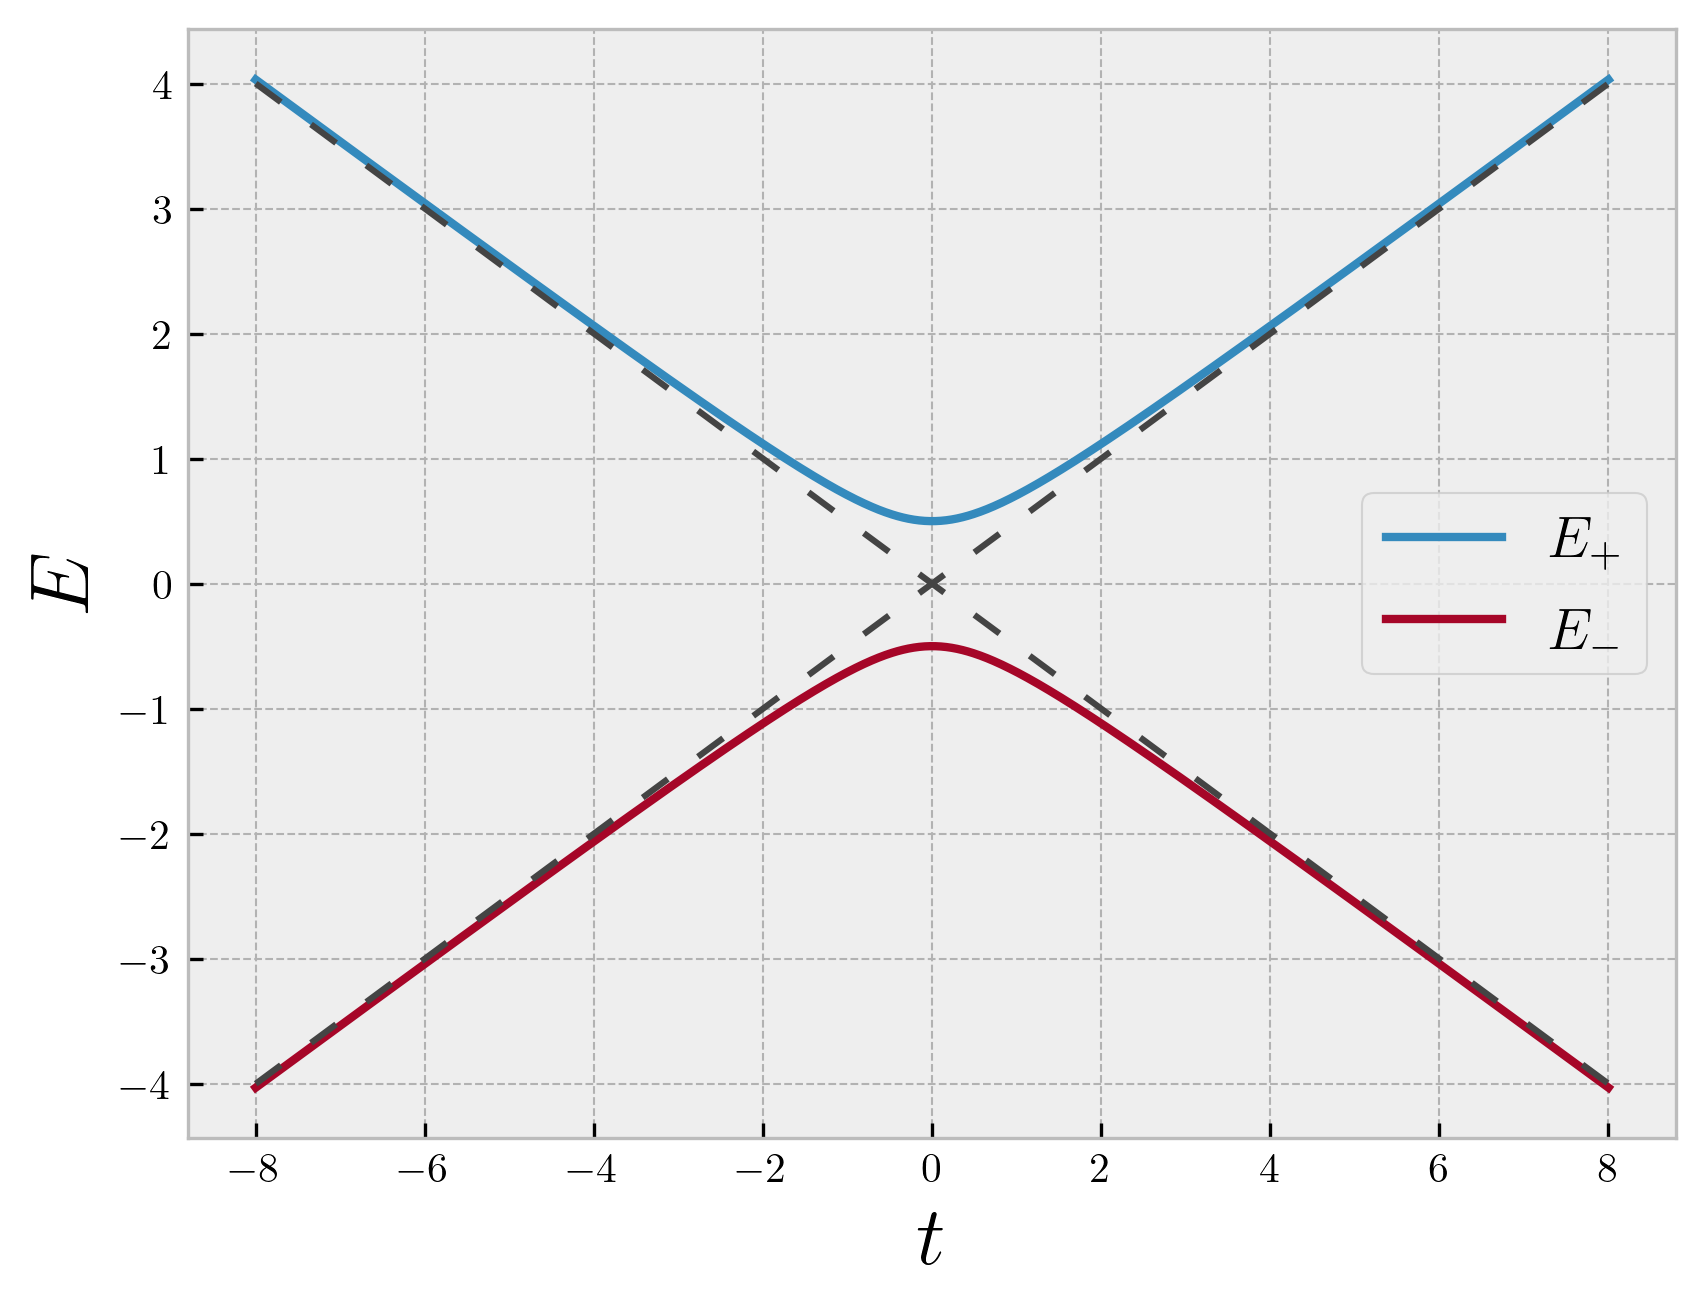
\includegraphics[scale=0.8]{figures/gap.png}
\caption{Energias do problema só fácil.}
\label{fig:gap}
\end{figure}
O que acontece quando $\Delta \to 0$ ?


\section{Aproximação?}
Nosso hamiltoniano pode ser aproximado por:
$$
\H =
\begin{bmatrix}
\alpha t/2 & \Delta/2 \\
\Delta^*/2 & -\alpha t/2
\end{bmatrix}.
$$
Vou tentar convencer vocês (e também a mim próprio) com alguns gráficos.

\section{Cálculo Real}

Schrödinger:
$$
\begin{bmatrix}
\dot{c}_1 \\ \dot{c}_2
\end{bmatrix}
= \frac{-i}{\hbar}
\begin{bmatrix}
\alpha t/2 & \Delta/2 \\
\Delta^*/2 & -\alpha t/2
\end{bmatrix}
\begin{bmatrix}
c_1 \\ c_2
\end{bmatrix}.
$$
Derivando, fazendo as contas e verificando que está tudo certo dimensionalmente:
\begin{ceqn}
\begin{align} \label{2ord}
\ddot{c}_1 + \qty(\frac{i\alpha}{2\hbar}+\frac{\alpha^2 t^2}{4\hbar^2}+\frac{\abs{\Delta}^2}{4\hbar^2})c_1 & = 0
\end{align}
\end{ceqn}
Quando $t \to \pm \infty$, temos que
$$
\H_{t \to \pm \infty} \approx
\begin{bmatrix}
\alpha t/2 & 0 \\
0 & -\alpha t/2
\end{bmatrix}.
$$
Este é o caso \textit{muito fácil}. Logo, esperamos fisicamente que, quando $t \to \pm \infty$, tenhamos que os módulos de $c_1$ e $c_2$ se estabilizem em uma constante. Em outras palavras:
$$
\existe \displaystyle{ \lim_{t \to \pm \infty} \abs{c_1(t)} = \abs{ c_1(\pm \infty)}}.
$$
Considerando então $t \gg 1$, escrevamos $c_1(t) = \abs{c_1} \, e^{-\frac{i}
{\hbar} \vphi(t)}$. Substituindo isso em (\ref{2ord}) temos
$$
\frac{1}{\hbar^2}\qty[\dot{\vphi}^2 + \frac{1}{4}\qty(\alpha^2t^2 + \abs{\Delta}^2)] +
\frac{i}{\hbar}\qty[\frac{\alpha}{2} - \ddot{\vphi}] = 0.
$$
Igualando as partes reais e imaginárias:
$$
\begin{cases}
\; \dot{\vphi} = \pm \frac{1}{2} \sqrt{\alpha^2t^2 + \abs{\Delta}^2}, \quad t \gg 1 \\
\; \ddot{\vphi} = \frac{\alpha}{2}
\end{cases}
$$
Com uma série de Taylor de primeira ordem para $\dot{\vphi}$:
$$
\dot{\vphi} = \frac{\alpha t}{2} \sqrt{1 + \frac{\abs{\Delta}^2}{\alpha^2t^2}} \approx
\frac{\alpha t}{2} + \frac{\abs{\Delta}^2}{4 \alpha t}, \quad t \to \pm \infty,
$$
obtemos que
\begin{ceqn}
\begin{align} \label{toinf}
\qty(\frac{\dot{c}_1}{c_1})_{t \to \pm \infty} &= -\frac{i}{\hbar} \qty(\frac{\alpha t}{2} + \frac{\abs{\Delta}^2}{4\alpha t}).
\end{align}
\end{ceqn}

\section{Cálculo Complexo}

Assumiremos que $\frac{\dot{c}_1}{c_1}$ tem uma extensão analítica para o semiplano complexo superior ou inferior. Com isso, temos os seguintes resultados para o valor principal de Cauchy:
$$
\int_{\Gamma} \frac{\dot{c}_1}{c_1}(z) \dd{z} = 0 \implies
$$
$$
\ln\qty[\frac{c_1(+\infty)}{c_1(-\infty)}] = \int_{-\infty}^\infty \frac{\dot{c}_1}
{c_1}(t) \dd{t} = - \int_{\Gamma_{\pm}} \frac{\dot{c}_1}{c_1}(z) \dd{z}
$$
onde $\Gamma_{\pm}$ é o arco de semicírculo superior ou inferior.

\n

\begin{obs}
\rm Note que $c_1(\pm \infty)$ não faz sentido, o que estamos interessados é $\abs{c_1(\pm \infty)}$. O que quero dizer acima é:
$$
\lim_{T \to \infty} \frac{c_1(T)}{c_1(-T)}.
$$
\end{obs}

\begin{figure}[H]
\centering
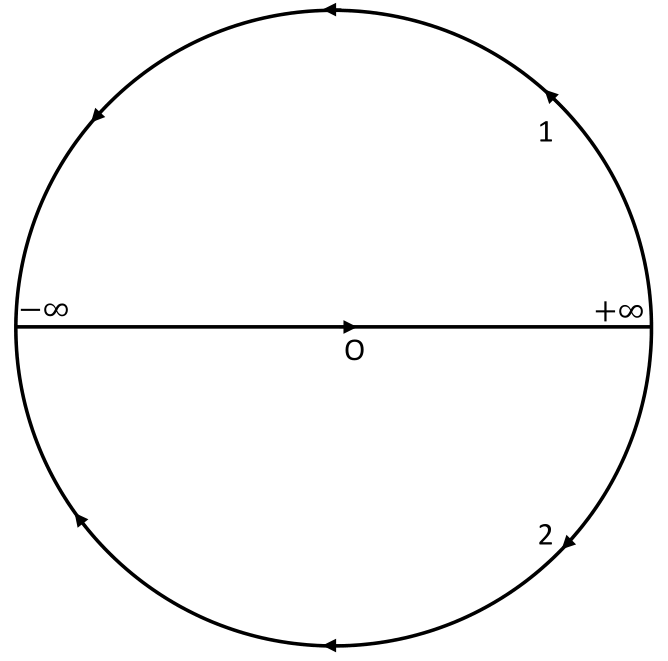
\includegraphics[scale=0.3]{figures/semicirculo.png}
\caption{Integração em algum dos semicírculos do plano complexo.}
\label{fig:semicirculo}
\end{figure}

Como $\frac{\dot{c}_1}{c_1}(z)$ é analítica por hipótese, pela equação (\ref{toinf}) podemos estender a fórmula para $z \in \C$
$$
\qty(\frac{\dot{c}_1}{c_1})_{z \to \pm \infty} = -\frac{i}{\hbar} \qty(\frac{\alpha z}{2} + \frac{\abs{\Delta}^2}{4\alpha z})
$$
e integraremos com $z = R e^{i\theta}$ e $\dd{z} = i R e^{i\theta} \dd{\theta}$:
$$
-\int_{\Gamma_{\pm}} \frac{\dot{c}_1}{c_1}(z) \dd{z} =
\frac{i}{\hbar} \int_{\Gamma_\pm} \qty(\frac{\alpha z}{2} + \frac{\abs{\Delta}^2}{4\alpha z}) \dd{z} =
$$
$$
\frac{i}{\hbar} \lim_{R \to \infty} \int_0^{\pm \pi}
\qty(\frac{\alpha R e^{i\theta}}{2} + \frac{\abs{\Delta}^2}{4\alpha R e^{i\theta}})
i R e^{i\theta} \dd{\theta} =
$$
$$
\frac{i}{\hbar} \lim_{R \to \infty} \int_0^{\pm \pi}
\qty(\frac{i \alpha R^2 e^{2i\theta}}{2}+\frac{i \abs{\Delta}^2}{4\alpha}) \dd{\theta} =
$$
$$
\frac{i}{\hbar} \lim_{R \to \infty} \qty[
\cancelto{0}{ \int_0^{\pm \pi} \frac{i \alpha R^2 e^{2i\theta}}{2} \dd{\theta} } +
\int_0^{\pm \pi} \frac{i \abs{\Delta}^2}{4\alpha} \dd{\theta} ] \implies
$$
$$
\ln\qty[\frac{c_1(+\infty)}{c_1(-\infty)}] =
\pm \frac{\pi \abs{\Delta}^2}{4 \hbar \alpha} \implies
$$
\n
$$
P_{\text{LZ}} = \abs{c_1(+\infty)}^2 =
\abs{c_1(-\infty)}^2 \exp(\pm\frac{\pi\abs{\Delta}^2}{2\hbar\alpha})
$$
Considerando o caso particular $\abs{c_1(-\infty)}^2 = 1$ e que $P_{\text{LZ}} \leq 1$,
devemos ter que
$$
P_{\text{LZ}} = \exp(-\frac{\pi\abs{\Delta}^2}{2\hbar\alpha}) = \exp[\frac{- \pi \abs{\Delta}^2}{2\hbar \, \dv{t}(\eps_1 - \eps_2)}].
$$
Perceba que isso correspondeu à integração no caminho $\Gamma_+$ (caminho \textcolor{RoyalBlue}{1} na Figura \ref{fig:semicirculo}).

\section{Referência}

Le Tuan Anh Ho, Liviu F. Chibotaru. \textit{A simple derivation of the Landau-Zener formula.}

\end{document}
